\PrestigeClass[\subsectionA][\subsubsection]{Avangion}
{Nothing on Athas is as dangerous as hope. Each of the destroyers of worlds set out to save or to restore. Will history remembers my hopes with the hopes of Gretch, Rajaat, and the architects of the Pristine Tower?}
{``Wisdom of Sorrow,'' by Oronis}
{
Having mastered both psionics and arcane magic, some of Athas' most powerful preservers seek out the mysteries of a metamorphosis that would change themselves into strange beings of gossamer wings and light.

As avangions, they can combine their mastery of the Way and arcane arts into psionic enchantments that some say counters dragon magic. Others say that the avangions bring a healing power, and that they come not to fight, but to return life to dying lands. Most sages have never heard of avangions, and would probably call them myth.
}
{d12}
{a}
{
Only an epic spellcaster with a fairly high manifester level can qualify to become an avangion. Avangions tend to dislike physical confrontation, so while a psychic warrior can qualify for this class, their combat-related powers don't add much. Because of the long and tedious processes in developing the metamorphosis, wilders likewise rarely become avangions. Some avangions take levels of cerebremancer to boost both their arcane and psionic skills.
}
{
\textbf{Skills:} \skill{Diplomacy} 11 ranks, \skill{Knowledge} (arcana) 23 ranks, \skill{Knowledge} (nature) 23 ranks, \skill{Knowledge} (psionics) 23 ranks, \skill{Psicraft} 23 ranks, \skill{Spellcraft} 23 ranks.

\textbf{Feats:} \feat{Iron Will}, \feat{Mind Over Body}, any two metamagic feats, and any two psionic feats.

\textbf{Spells:} Able to cast 9th-level arcane spells.

\textbf{Psionics:} Able to manifest 7th-level powers.

\textbf{Special:} Must be a preserver.

\textbf{Special:} Must perform a special ritual (see \hyperref[Avangion Metamorphosis]{Avangion Metamorphosis}).
}
{
\skill{Concentration} (Con), \skill{Craft} (Int), \skill{Decipher Script} (Int), \skill{Diplomacy} (Cha), \skill{Knowledge} (all skills, taken separately) (Int), \skill{Psicraft} (Int), \skill{Sense Motive} (Wis), and \skill{Spellcraft} (Int).
}
{2}
{\WarriorTable[ll *{3}{Z{12mm}} L]}
{
 1 & +1  & +2 & +2 & +2 & Continued advancement, divine rank, spell-like abilities \\
 2 & +2  & +3 & +3 & +3 & Natural armor, resistance, wings \\
 3 & +3  & +3 & +3 & +3 & DR 10/metal and magic \\
 4 & +4  & +4 & +4 & +4 &  \\
 5 & +5  & +4 & +4 & +4 & DR 15/cold iron and magic \\
 6 & +6  & +5 & +5 & +5 &  \\
 7 & +7  & +5 & +5 & +5 & Wisdom increase \\
 8 & +8  & +6 & +6 & +6 & DR 20/cold iron and epic, Wisdom increase \\
 9 & +9  & +6 & +6 & +6 & Wisdom increase \\
10 & +10 & +7 & +7 & +7 & Wisdom increase \\
}
{
\textbf{Continued Advancement:} When a new avangion level is attained, the character gains new spells per day as if he had also attained a level in any one arcane spellcasting class he belonged to before he added the prestige class. He gains additional power points per day and access to new powers as if he had also gained a level in any one manifesting class he belonged to previously. He does not, however, gain any other benefit a character of either class would have gained (bonus metamagic, metapsionic, or item creation feats, psicrystal special abilities, and so on). This essentially means that he adds the level of avangion to the level of whatever other arcane spellcasting class and manifesting class the character has, then determines spells per day, caster level, power points per day, powers known, and manifester level accordingly.

If a character had more than one arcane spellcasting class or more than one manifesting class before he became an avangion, he must decide to which class he adds each level of avangion for purpose of determining spells per day, caster level, power points per day, powers known, and manifester level.

\textbf{Divine Rank:} An avangion is considered a demigod. He can grant spells and perform a few deeds that are beyond mortal limits. He is immune to the effects of aging and never dies of ``natural causes.'' For more information, see \hyperref[Divine Rank]{Divine Rank}.

\textbf{Spell-Like Abilities:} A dragon gains the ability to understand and speak any language, as per the \spell{tongues} spell. This spell-like ability is always considered active.

\begin{figure*}[b!]
\centering
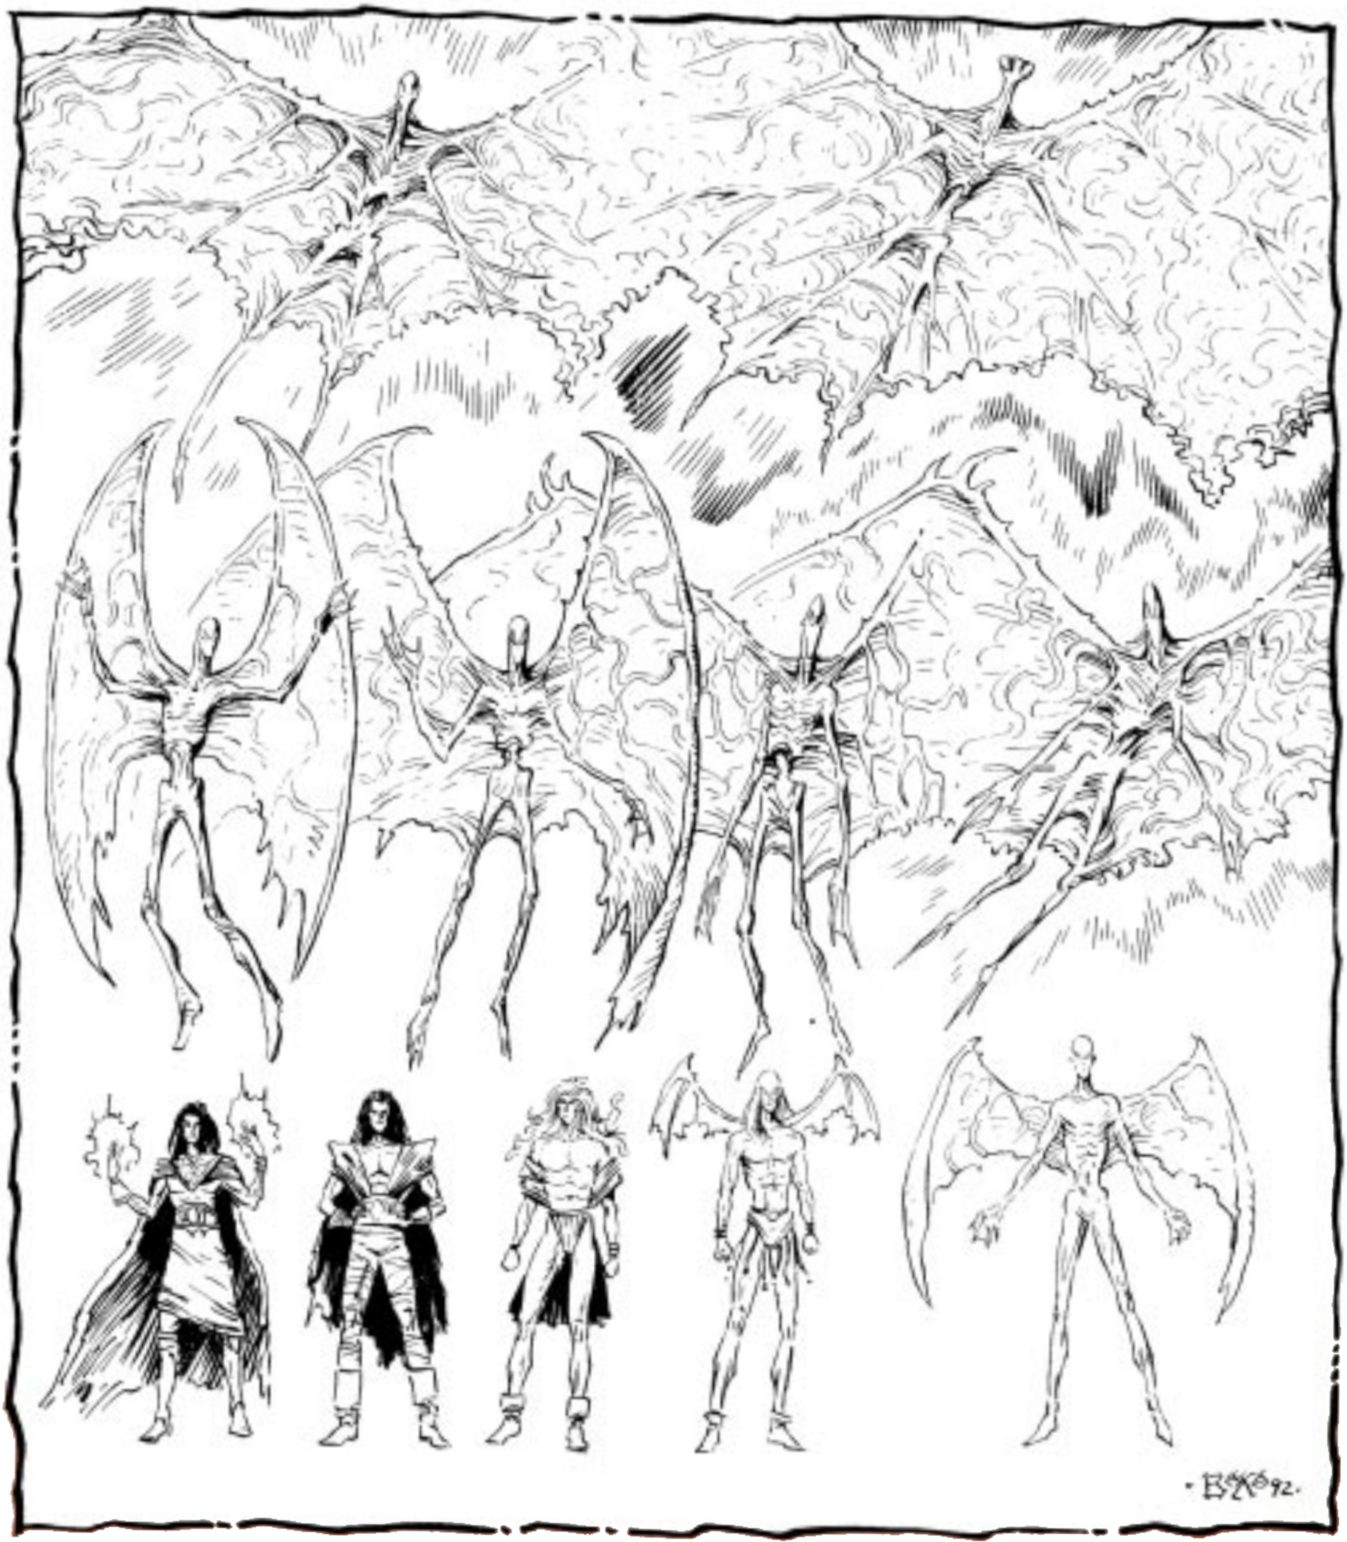
\includegraphics[width=\textwidth]{images/avangion-1.png}
\WOTC
\end{figure*}

\textbf{Increased Size:} At 2nd level and every three levels thereafter (5th and 8th level), a dragon increases in size by one category. At each size increase, the dragon improves his Strength score by 8, and his Constitution score by 4. The size indicated at the table is for Medium dragons. Small and Large dragons increase the size by one category normally. Small Dragons that become Medium improve Strength as indicated, as this is not a normal monster progression. Colossal dragons cannot increase further in size.

\textbf{Improved Speed (Ex):} At 4th level, a dragon increases his land speed by 6 meters.

\textbf{Natural Armor:} At 4th level, tough scales, now everywhere but the underbelly and the underside of its limbs, grant a dragon natural armor equal to its level + his Intelligence modifier.

\textbf{Damage Reduction:} At 5th level, a dragon's gains damage reduction 10/metal and magic. So attacks from weapons that are not made of metal have their damage reduced, even if the weapon has an enhancement bonus. Only metal weapons with an enhancement bonus can ignore this damage reduction. Damage reduction can reduce damage to 0 but not below 0.

At 8th level, this damage reduction improves to 20/metal and epic. Only attacks with metal weapons with an enhancement bonus of +6 or better can ignore this damage reduction.

\textbf{Resistance (Su):} At 6th level, a dragon gains spell resistance and power resistance equal to 12 + dragon's HD.

\textbf{Breath Attack (Su):} At 7th level, a dragon can use its breath weapon, a cone of superheated sand 15 meters long. The cone deals 10d12 points of damage. A blast from a breath weapon always starts at any intersection adjacent to the dragon and extends in a direction of the dragon's choice. The creatures caught in the area can attempt Reflex saves to take half damage. The save DC against a breath weapon is 10 + dragon's HD + dragon's Con modifier.

At 9th level, the dragon's breath attack increases its damage to 20d12.

\textbf{Draconic Perfection:} By obtaining the 10th level, the dragon's type changes to Dragon. All of his hit dice become d12. He increases in size by one last time, and his natural attacks increase their damage because of it. His flight speed improves to 45 meters with average maneuverability. His breath attack damage increases to 25d12.

\subsubsection{Avangion Metamorphosis}
\label{Avangion Metamorphosis}

In order to receive the benefits of the prestige class, a character must perform a ritual to change their body. This ritual depends on the level in which the character wants to obtain. Although the experience points have been earned (or the number of sessions have been passed), the preserver gains no benefits of his new level until after the ritual is complete.

The ritual functions as a special spell of at least 9th-level that consumes all power points from the caster. It has the verbal, somatic, and material components of a normal spell. Besides, some transformations require a arcane focus.

\textbf{Low Level (1st, 2nd, and 3rd levels):} The preserver leaves the company of his fellows and seeks isolation. In this isolation period, the preserver must gather physical remains of the enemies of life, usually those of high-level defilers---their bodily remains, destructive belongings or artifacts, ash from their spellcasting, etc. The spell must be cast at night, beneath the light of both Athasian moons.

\textit{Spell Level:} 9th-level.

\textit{Casting Time:} 6 hours.

\textit{Material Component:} Six bodies or belongings of defilers capable of casting 9th-level spells, or ashes of defiling radius of 9th-level spells cast by six different defilers. These defilers must have been defeated by the preserver in a single combat.

\textbf{Middle Level (4th, 5th, and 6th levels):} The preserver must attain absolute isolation---any contact with intelligent beings who aren't foes to be defeated negates the spell preparation. During the preparation time, the caster must receive at least three gifts from powerful good creatures. Usually, these gifts are rewards for completing extremely important or dangerous goals determined prior to the preparation of the spell. The spell must be cast in a forest or an area of dense vegetation. At the time of casting, there must be living vegetation for at least 1.5 kilometers in all directions, untainted by defiler ash or evil creatures.

\textit{Spell Level:} 10th-level.

\textit{Preparation Time:} Special (see above).

\textit{Casting Time:} 12 hours.

\textit{Material Components:} At least three gifts from good creatures with at least 20 Hit Dice.

\textit{Arcane Focus:} A single tree or bush personally saved by the preserver from defiler magical destruction.

\textbf{High Level (7th, 8th, and 9th levels):} Unlike previous advancements, the preserver has no calling toward isolation at high levels. Instead, he must collect a core group of companions, no fewer than eight in number and of at least 10 ECL each. All companions must be of good alignment. The preserver must spend the preparation time with these characters. During the casting of the spell, the preserver must have the aid of a single companion for the entire length of the ritual. If the companion is of non-good alignment, the spell fails and the companion is slain. Companions cannot repeat the process with a single preserver, at each level the preserver must find new companions.

\textit{Spell Level:} 10th-level.

\textit{Preparation Time:} 1 year.

\textit{Casting Time:} 24 hours.

\textit{Material Component:} A single gift from each of the companions in the core group (see above).

\textbf{Final Level (10th level):} The preserver must make an area of lush vegetation (crops, scrubs, forest, or any combination) at least 8 kilometers in diameter. The preparation time is the time it takes the preserver to create these lush lands. At the time of casting, the lush lands must be free of evil creatures. The preserver and the material components disappear after casting the spell. The preserver returns in his final avangion form to the glass case after 2d6 months. If the glass case is damaged in the meantime, the avangion is lost to oblivion.

\textit{Spell Level:} 10th-level.

\textit{Preparation Time:} Special (see above).

\textit{Casting Time:} 1 full round.

\textit{Material Components:} A single diamond worth at least 30,000 cp, and a stone tomb large enough to hold the preserver's body.

\textit{Arcane Focus:} A perfectly sealed glass case built around the tomb.
}